%%%%%%%%%%%%%%%%%%%%%% Version Information %%%%%%%%%%%%%%%%%%%%%%%%%%% 
% This LaTeX2e thesis template is based on the nuthesis-template
% provided by Miguel A. Lerma. It was renamed and edited to meet the
% requirements given in the Thesis-Dissertation Instructions of the
% School of Graduate Studies of Case Western Reserve University by
% Initial Version: Frank Ernst (Dr. rer. nat. habil., Professor). 
%   Version dated 2006-08-23.
% Latest Version: Roger French (Professor). 
%  SDLE Center Authors: Nicholas Wheeler, Myles Murray, Heather Lemire
%  Version dated 2015
%%%%%%%%%%%%%%%%%%%%%%%%%%%%%%%%%%%%%%%%%%%%%%%%%%%%%%%%%%%%%%%%%%%%%% 

%%%%%%%%%%%%%%%%%%%%%%%%%%%%%% DISCLAIMER %%%%%%%%%%%%%%%%%%%%%%%%%%%%
% The author of the thesis remains responsible for fulfilling all
% requirements.
%%%%%%%%%%%%%%%%%%%%%%%%%%%%%%%%%%%%%%%%%%%%%%%%%%%%%%%%%%%%%%%%%%%%%%

%%%%%%%%%%%%%%%%%%%%%%%%%%%%% DESCRIPTION %%%%%%%%%%%%%%%%%%%%%%%%%%%%
% cwru-cse-thesis.tex is the master file that compiles the whole thesis.
% Individual chapter files located in 'content' folder
% Appendix files located in 'app' folder
% bibtex file for references located in 'refs' folder
% figure files go in the 'figs' folder
% the 'input' folder has style files for tex compiling
%%%%%%%%%%%%%%%%%%%%%%%%%%%%%%%%%%%%%%%%%%%%%%%%%%%%%%%%%%%%%%%%%%%%%%

\documentclass[help,12pt,onepage,reqno]{input/CWRU-Thesis}



%%%%%%%%%%%%%
% EQUATIONS %
%%%%%%%%%%%%%

% ArgMin
\DeclareMathOperator*{\argmin}{\arg\!\min}

% ArgMax
\DeclareMathOperator*{\argmax}{\arg\!\max}

% Custom colors
\usepackage{color}
\definecolor{deepblue}{rgb}{0,0,0.5}
\definecolor{deepred}{rgb}{0.6,0,0}
\definecolor{deepgreen}{rgb}{0,0.5,0}
%\definecolor{coolblue}{HTML}{101094}

\usepackage{listings}

\definecolor{codebg}{RGB}{238,238,238}

% Python style for highlighting
\newcommand\pythonstyle{\lstset{
    language=Python,
    basicstyle=\ttm,
    otherkeywords={},             % Add keywords here
    keywordstyle=\ttm\color{coolblue},
    emph={MyClass},          % Custom highlighting
    emphstyle=\ttm\color{deepred},    % Custom highlighting style
    stringstyle=\color{deepgreen},
    frame=tb,                         % Any extra options here
    framesep=10pt,
    framexleftmargin=10pt,
    backgroundcolor=\color{codebg},
    rulecolor=\color{codebg},
    aboveskip=15pt,
    belowskip=15pt,
    showstringspaces=false            % 
}}


% Python environment
\lstnewenvironment{python}[1][] {
    \pythonstyle
    \lstset{#1}
}{}

% \setmonofont[Color={0019D4}]{Courier New}


% Python for external files
\newcommand\pythonexternal[2][]{{
\pythonstyle
\lstinputlisting[#1]{#2}}}

% Python for inline
\newcommand\pythoninline[1]{{\pythonstyle\lstinline!#1!}}

% Path of images
%\graphicspath{ {./figs} }

%%%%%%%%%%%%%%%%%%%%%%%%%%%%%%%%%%%%%%%%%%%%%%%%%%%%%%%%%%%%%%%%%%%%%%%%%%%%%%%%%%%%%%%%%%%%%%%%%%%%



% Uncomment *one* of the following lines if you are tired of TeX's
% Computer Modern fonts:
\usepackage{fourier} 
%\usepackage{mathpazo}
%\usepackage{mathptmx}

% Graphics.
\usepackage[pdftex]{graphicx}
\usepackage{subfig}
\usepackage{pdflscape} % landscape environment
%\usepackage{subfigure}
\usepackage{longtable}

% The following makes graphicx work with pdf and jpg files. Files with
% same names and different extensions will be recognized in sequential
% order.
\DeclareGraphicsExtensions{.png, .jpg, .pdf} 

% PDFPages imports entire PDF pages.
%\usepackage[draft]{pdfpages} % not sure that this actually works
\usepackage[final]{pdfpages}

% Sets pdftex to included versions up to 1.6
%\pdfminorversion=6
\pdfoptionpdfminorversion=6

% Chapterbib enables separate bibliographies after each chapter.
%\usepackage[sectionbib]{chapterbib}
%\usepackage[rootbib]{chapterbib}

\usepackage{verbatim} %for comment environment

% % to allow underscore in text, doesn't work if you actually use
% % underscores in the latex doc
% \usepackage{underscore}
% \begingroup
%   \lccode`\~=`\_
% \lowercase{\endgroup
%   \pdfstringdefDisableCommands{\let~\relax}%
% }

% Wrapfig wraps tables and figures.
\usepackage{wrapfig} 
\usepackage{multirow}

% footnotes in tables
\usepackage{threeparttable}
% \usepackage{footnote}
% \makesavenoteenv{tabular} % makes tables handle footnotes correctly

% Your packages can go here:
\usepackage{input/KL-Typing-Aids}

% Author and title
\author{\uppercase{Peng Xu}}
\title{Cooperative Control of Autonomous Vehicle on Highways}

\degree{Master of Science}  
% Default: Doctor of Philosophy.

%\adviser{Dr. Roger H. French}     
% Optional -- Default: Empty.

\department{\deecs}     
% No Default.

\graduationmonth{May}      
% The default is January, May, or August depending on current date.

\graduationyear{2018}
% Default: current year.
% CAUTION: next January could be *next* year.


%\includeonly{05-Background, 06-Methods}
% Use \includeonly to select the chapters to include if you are using
% the \include command below. This way you can latex only a the part
% you are working on, which is faster than latexing the entire thesis.

% Margin kerning.
\input input/protcode.tex

%	%------------------- Markup
	% new commands for markup/editing purposes
	% make a \newcommand for your self, this rhf set is for Roger (rhf) and Dan (dmd)
	\usepackage{xcolor}
	\usepackage{ulem}
		% color names = red, green, blue, cyan, magenta, yellow, black, gray, white,  
		%   darkgray, lightgray, brown, lime, olive, orange, pink,  purple, teal, violet
		%   
			%-------------------------
				% rhf = Roger markup
			\newcommand{\rhf}{\textcolor{red}} % for rhf = Roger is red text
			\newcommand{\rhfcomm}[1]{
			       \colorbox{yellow}{#1} % Roger is yellow highlight
			       }
			\newcommand{\rhfstr}[1]{
				\sout{#1} %Roger's strikethrough
			}
			%-------------------------
			
\usepackage{hyperref} % enables hyper links in the document's pdf file output

\begin{document}%%%%%%%%%%%%%%%%%%%%%%%%%%%%%%%%

%Margin kerning.
\setprotcode \font
{\it \setprotcode \font}
{\bf \setprotcode \font}
{\bf \it \setprotcode \font}

% % To turn off hyphen protrusion at end of line, set to "0".
\pdfprotrudechars=1 

\frontmatter
%\pagenumbering{roman}

% Title page.
\maketitle		

% Page for signatures of the committee members.
%For the final turn in, you do not need this page signed, just dated.
% to date this page, cludgy way to do it is replace Signature/Date with the Date
%Found in the CWRU-thesis.cls file, line 327
\signaturepage
\sign[Adviser]{Dr. Wyatt Newman}{Chair}{\deecs}
\sign{Dr. M. Cenk Cavusoglu}{Member}{\deecs}
%\sign{\fe}{Member}{\deecs} %if pre programed can use short name thing

% Copyright page. You do not need a copyright page unless
% you are applying for a copyright.
%\copyrightpage 

% Dedication page (optional). Please indicate linebreaks by "\\".
\dedication{Dedicated to *your\\dedication message goes here*}

% Preface (optional).
%\preface
%\input{03-Preface}

% Table of Contents will be automatically generated and placed here.
\tableofcontents

% List of Tables and List of Figures will be automatically generated
% and placed here.
\listoftables	
%\subfiglabelskip=0pt % suppresses spacing after empty subfiglabel set
                     % to 0pt; for use with subfigure.sty
\listoffigures		

% Acknowledgements (optional).
\acknowledgements
\begin{sloppypar}
\section{Acknowledgements}


\end{sloppypar}

% Abstracts must not exceed 350 words in dissertations and 150
% words in other theses.
\abstract
\begin{sloppypar}
\section{Abstract}


The present paper describes a study that aims at assessment of driver behavior in response to new technology, particularly Adaptive Cruise Control Systems (ACCs), as a function of driving style. In this study possible benefits and drawbacks of Adaptive Cruise Control Systems (ACCs) were assessed by having participants drive in a simulator. The four groups of participants taking part differed on reported driving styles concerning Speed (driving fast) and Focus (the ability to ignore distractions), and drove in ways which were consistent with these opinions. The results show behavioral adaptation with an ACC in terms of higher speed, smaller minimum time headway and larger brake force. Driving style group made little difference to these behavioral adaptations. Most drivers evaluated the ACC system very positively, but the undesirable behavioral adaptations observed should encourage caution about the potential safety of such systems.

\newpage
\end{sloppypar}
%can you run bibliography on abstract?
%\bibliographystyle{plainnat}
%\bibliography{my_references}
 

\mainmatter             
\pagenumbering{arabic} 

% Change hyperlink color to a bluish hue that is fairly visible, but
% not disturbing in long lists of references, and will also print well
% in black and white. Up to this point, the hyperlink color was black
% (default) to avoid that the tables of contents, figures, and tables
% entirely appear in color.
\definecolor{felinkcolor}{rgb}{0,0,0.5}

\chapter{Introduction}


\section{Motivation and Background}

% Autonomous Vehicle

Modern technologies have the potential to create a paradigm shift in the vehicle-driver relationship with advanced automation changing the driver role from "driving" to "supervising". To design new driver environments that caters for these emerging technologies, traditional approaches identify current human and technical constraints to system efficiency and create solutions accordingly. However, there are two reasons why such approaches are limited within the technologically-evolving automotive domain. First, despite significant progress in the development of system theory and methods, the application of these methods is largely constrained to the existence of a current system. Second, there are few structured approaches for using the analysis results to support design. In this paper, an attempt is made to overcome these challenges by developing and implementing a method for analyzing and designing a highly autonomous commercial vehicle. 

An autonomous vehicle has great potential to improve driving safety, comfort and efficiency and can be widely applied in a variety of fields, such as road transportation, agriculture, planetary exploration, military purpose and so on \cite {WANG2015727}. The past three decades have witnessed the rapid development of autonomous vehicle technologies, which have attracted considerable interest and efforts from academia, industry, and governments. Particularly in the past decade, contributing to significant advances in sensing, computer technologies, and artificial intelligence, the autonomous vehicle has become an extraordinarily active research field. During this period, several well-known projects and competitions for autonomous vehicles have already exhibited autonomous vehicles' great potentials in the areas ranging from unstructured environments to the on-road driving environments \cite{AutonomousStructured} \cite{DrivingUrban2008}.

% Highway Driving

Complex functions like highly automated driving with combined longitudinal and lateral control will definitely appear first on highways, since traffic is more predictable and relatively safe there (one-way traffic only, quality road with relative wide lanes, side protections, good visible lane markings, no pedestrians or cyclists, etc.). As highways are the best places to introduce hands-free driving at higher speeds, one could expect a production vehicle equipped with a temporary autopilot or in other words automated highway driving assist function as soon as the end of this decade. 

Automated highway driving means the automated control of the complex driving tasks of highway driving, like driving at a safe speed selected by the driver, changing lanes or overtaking front vehicles depending on the traffic circumstances, automatically reducing speed as necessary or stopping the vehicle in the right most lane in case of an emergency. Japanese Toyota Motor have already demonstrated their advanced highway driving support system prototype in real traffic operation. The two vehicles (shown on Figure 83) communicate each other, keeping their lane and following the preceding vehicle to maintain a safety distance. (Source: [70])



% Adaptive Cruise Control

In this paper, we are aiming for an autonomous driving system allowing the vehicle to smartly choose the driving behaviors, such as adjusting the speed and changing the lane. In fact, Adaptive cruise control (ACC), a radar-based system, has been designed to enhance driving comfort and convenience by relieving the need to continually adjust the speed to match that of a preceding vehicle. The system slows down when it approaches a vehicle with a lower speed, and the system increases the speed to the level of speed previously set when the vehicle upfront accelerates or disappears (e.g., by changing lanes). Traditional methods have proved the reliability in several cases though the use is still quite limited and only for expected scenarios. While, currently, artificial intelligence especially deep reinforcement learning is aggressively expanding the border of human's imagination and machine's autonomy. Thus, a new highway adaptive cruise control (HACC) is proposed for autonomous vehicles with the help of deep reinforcement learning.

\section{Literation Review}

The past few years have seen many breakthroughs using reinforcement learning (RL). The company DeepMind combined deep learning with reinforcement learning to achieve above-human results on a multitude of Atari games and, in March 2016, defeated Go champion Le Sedol four games to one. Though RL is currently excelling in many game environments, it is a novel way to solve problems that require optimal decisions and efficiency, and will surely play a part in machine intelligence to come.

% The rise of Deep Q Learning

Google's DeepMind published its famous paper Playing Atari with Deep Reinforcement Learning \cite {Mnih2015AtariNature}, in which they introduced a new algorithm called Deep Q Network (DQN for short) in 2013. It demonstrated how an AI agent can learn to play games by just observing the screen without any prior information about those games. The result turned out to be pretty impressive. This paper opened the era of what is called "deep reinforcement learning", a mix of deep learning and reinforcement learning.

% Reinforcement Learning
Reinforcement Learning is a type of machine learning that allows you to create AI agents that learn from the environment by interacting with it. Just like how we learn to ride a bicycle, this kind of AI learns by trial and error. As seen in Fig. \ref {fig:deepmind}, the brain represents the AI agent, which acts on the environment. After each action, the agent receives the feedback. The feedback consists of the reward and next state of the environment. The reward is usually defined by a human. If we use the analogy of the bicycle, we can define reward as the distance from the original starting point.

\begin{figure}[h] 
\centering
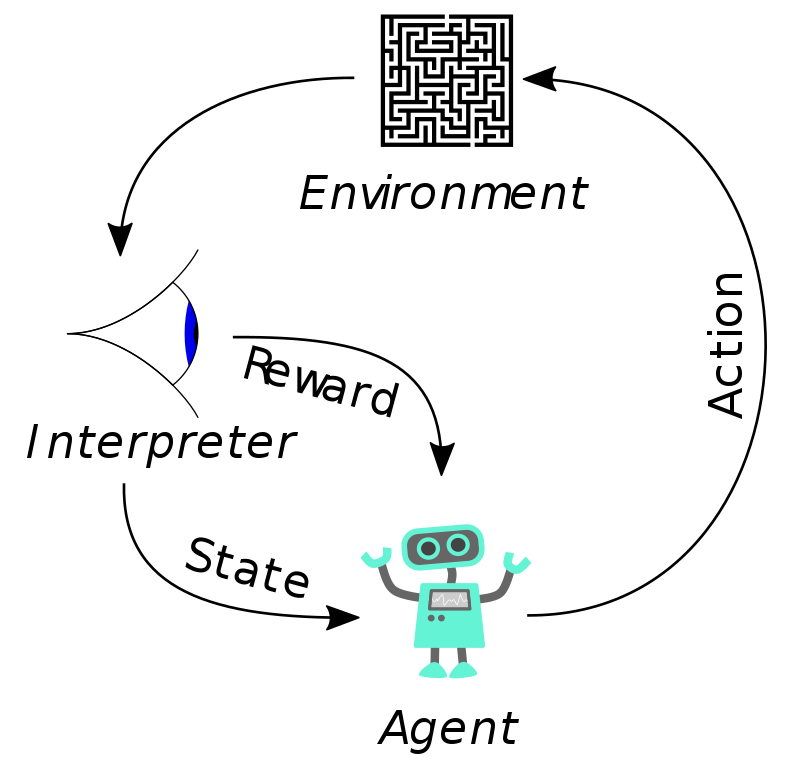
\includegraphics[width=0.5\textwidth]{figs/ch1/Reinforcement_learning_diagram}
\caption{How an agent interacts with the environment.}
\label{fig:deepmind}
\end{figure}

Standard model-based methods for robotic manipulation might involve estimating the physical properties of the environment, and then solving for the controls based on the known laws of physics \cite{OK-Robot-1987} \cite{Predictive2014} \cite{PlanningFramework2012}. This approach has been applied to a range of problems. Despite the extensive work in this area, tasks like pushing an unknown object to a desired position remain a challenging robotic task, largely due to the difficulties in estimating and modeling the physical world \cite{IROS2016}. Learning and optimization-based methods have been applied to various parts of the state-estimation problem, such as object recognition \cite{Visual1995}, pose registration \cite{ObjectRecognition2009}, and dynamics learning \cite{DynamicsDoor2013}.

However, estimating and simulating all of the details of the physical environment is exceedingly difficult, particularly for previously unseen objects, and is arguably unnecessary if the end goal is only to find the desired controls. For example, simple rules for adjusting motion, such as increasing force when an object is not moving fast enough, or the gaze heuristic \cite{FieldersNature2003}, can be used to robustly perform visuomotor control without an overcomplete representation of the physical world and complex simulation calculations. Our work represents an early step toward using learning to avoid the detailed and complex modeling associated with the fully model-based approach.

Several works have used deep neural networks to process images and represent policies for robotic control, initially for driving tasks \cite{AutonomousLand1989} \cite{LongrangeVision2009}, later for robotic soccer \cite{RobotSoccer2009}, and most recently for robotic grasping \cite{Grasp2016} \cite{RooticGrasping2016} and manipulation \cite{Visuomotor2016}. Although these model-free methods can learn highly specialized and proficient behaviors, they recover a task-specific policy rather than a flexible model that can be applied to a wide variety of different tasks. The high dimensionality of image observations presents a substantial challenge to model-based approaches, which have been most successful for low-dimensional non-visual tasks \cite{PolicySearch2011} such as helicopter control \cite{HeliNg2007}, locomotion \cite{Trajectory2012}, and robotic cutting \cite{Deepmpc2015}. Nevertheless, some works have considered modeling high-dimensional images for object interaction. For example, Boots et al. \cite{Predictive2014} learn a predictive model of RGB-D images of a robot arm moving in free space.

% CACC

A lot of related work has been done in recent years in the design of CACC systems. Regarding the vehicle-following controller, Hallouzi et al. [8] did some research as part of the CarTalk 2000 project. These authors worked on the design of a longitudinal CACC controller based on vehicle-to-vehicle communication. They showed that inter-vehicle communication can help reduce instability of a platoon of vehicles. In the same vein, Naranjo and his colleague [14] worked on designing a longitudinal controller based on fuzzy logic. Their approach is similar to what we did with reinforcement learning for our low-level controller. Forbes has presented a longitudinal reinforcement learning controller [5] and compared it to a hand-coded following controller. He showed that the hand-coded controller is more precise than its RL controller but less adaptable in some situations. However, Forbes did not test explicitly communication between vehicles to improve its longitudinal controller to a multi-vehicle environment (which will be the focus of our future work). Our approach will also integrate our low-level controllers with a high-level multiagent decision making algorithm, which was not part of Forbes' work.

Regarding the reinforcement learning in a vehicle coordination problem, Unsal, Kachroo and Bay \cite{CACC1999} have used multiple stochastic learning automata to control the longitudinal and lateral path of a vehicle. However, the authors did not extend their approach to the multi-agent problem. In his work, Pendrith \cite{DistributedRL-Traffic2000} presented a distributed variant of Q-Learning (DQL) applied to lane change advisory system, that is close to the problem described in this paper. His approach uses a local perspective representation state which represents the relative velocities of the vehicles around. Consequently, this representation state is closely related to our 1-partial state representation. Contrary to our algorithms, DQL does not take into account the actions of the vehicles around and updates Q-Values by an average backup value over all agents at each time step. The problem of this algorithm is the lack of learning stability.

On the other hand, our high level controller model is similar to Partially Observable Stochastic Games (POSG). This model formalizes theoretically the observations for each agent. The resolution of this kind of games has been studied by Emery-Montermerlo \cite{GameControl2005}. This resolution is an approximation using Bayesian games. However, this solution is still based on the model of the environment, unlike our approach which does not take into account this information explicitly since we assume that the environment is unknown. Concerning the space search reduction, Sparse Cooperative Q-Learning \cite{Sparse2004} allows agents to coordinate their actions only on predefined set of states. In the other states, agents learn without knowing the existence of the other agents. However, unlike in our approach, the states where the agents have to coordinate themselves are selected statically before the learning process. The joint actions set reduction has been studied by Fulda and Ventura who proposed the Dynamic Joint Action Perception (DJAP) algorithm \cite{JointAction2003}. DJAP allows a multi-agent Q-learning algorithm to select dynamically the useful joint actions for each agent during the learning. However, they concentrated only on joint actions and they tested only their approach on problems with few states.

Introducing communication into decision has been studied by Xuan, Lesser, and Zilberstein \cite{Multi-agentCooperation2001} who proposed a formal extension to Markov Decision Process with communication where each agent observes a part of the environment but all agents observe the entire state. Their approach proposes to alternate communication and action in the decentralized decision process. As the optimal policy computation is intractable, the authors proposed some heuristics to compute approximation solutions. The main differences with our approach is the implicit communication and the model-free learning. More generally, Pynadath and Tambe \cite{Communicative2002} have proposed an extension to distributed POMDP with communication called COM-MTDP, which take into account the cost of communication during the decision process. They presented complexity results for some classes of team problems. As Xuan, Lesser, and Zilberstein \cite{Multi-agentCooperation2001}, this approach is mainly theoretical and does not present model-free learning. The locality of interactions in a MDP has been theoretically developed by Dolgov and Durfee \cite{Makov2004}. They presented a graphical approach to represent the compact representation of a MDP. However, their approach has been developed to solve a MDP and not to solve directly a multi-agent reinforcement learning problem where the transition function is unknown.


\section{Thesis Outline}

The goal of this thesis is to provide operational specifications for the development of a level 4 capable AVRP. This section will present the chapters and subsections of this thesis and provide a brief summary of those sections.

Chapter 2 details the system specifications required to develop an AVRP, based off feedback from faculty and researchers at Virginia Tech.
\begin{itemize}
\item \textbf {Section 2.1 Interdisciplinary Design Needs:} Looks at the feedback given by faculty and researchers at Virginia Tech and what kinds of research they would like to utilize an AVRP for. Breaks down the research desires into the basic needs for an AVRP. Some of the feedback is broken down with more background information.
\end{itemize}

Chapter 3 dives into the hardware and sensing side of an AVRP and lays out a discussion of the technology needed, such as DBW, navigation, sensing, communication, computing, power bus, and external mounting racks. It then reviews additional design considerations that need to be taken into consideration when designing an AVRP. Chapter 3 is laid out as follows:
\begin{itemize}
\item \textbf {Section 3.1 Drive By Wire:} Discusses the DBW system and significant design parameters to be considered. Lays out the specifications of the by wire system on a base platform at Virginia Tech. Presents a high level overview of DBW system.
\item \textbf {Section 3.2 Navigation:} Discusses different combinations for navigation, such as GPS/ INS and GPS/IMU, and some of the characteristics associated with each, as well as navigation via dead reckoning. Correction techniques such as DGPS and DGPS with RTK are reviewed. Hardware mounting is briefly mentioned.
\item \textbf {Section 3.3.1 LIDAR:} Discusses how LIDAR works. 2D and 3D LIDAR is discussed. Discusses certain characteristics such as range, accuracy, field of view, number of re- turns, intensity, advantages and disadvantages. Reviews possible mounting locations.
\item \textbf {Section 3.3.2 Radar:} Discusses how radar works and its usefulness on an AVRP. Talks about the different operation frequencies used in autonomy and how they affect performance, as well as other advantages and disadvantages. Possible mounting locations are discussed.
\item \textbf {Section 3.3.3 Ultrasonic:} Discusses the use of ultrasonic sensors and their advantages and disadvantages. Reviews their range and mounting locations.
\item \textbf {Section 3.3.4 Cameras:} Discusses different camera types and capability they bring to an AVRP. Goes over camera specifications for consideration. Reviews potential mounting locations.
\item \textbf {Section 3.3.5 Wheel Speed and Steering Angle Sensors: }Discusses wheel encoders and steering angle sensors and how they complement other sensing and systems.
\item \textbf {Section 3.4.1 Communication:} Presents different communication buses for intra-vehicle communication. Provides an overview, specs, and explanation of an AVRP communication bus structure. Reviews the need for an emergency stop system.
\item \textbf {Section 3.4.2 Computers:} Addresses computing for the end users by presenting bench- marks and guide posts for consideration when determining computational needs for the end user of an AVRP.
\item \textbf {Section 3.5 Base Sensor Suite Design:} Specs out the base sensor suite for an AVRP and the capabilities it allows for the AVRP without user added sensors.
\item \textbf {Section 3.6 Power Bus:} Discusses AVRP power bus layout to provide power to all internally and externally mounted hardware and sensors. Provides an estimate of power need for base sensor suite and an example sensor suite.
\item \textbf {Section 3.7.1 Front Universal Mounting Racks:} Reviews details and modifications made for adding front universal mounting rack to AVRP.
\item \textbf {Section 3.7.2 Rear Universal Mounting Racks:} Reviews details and modifications made for adding rear universal mounting rack to AVRP.
\item \textbf {Section 3.7.3 Roof Universal Mounting Racks:} Reviews details and modifications made for adding roof top universal mounting rack to AVRP.
\item \textbf {Section 3.7.4 Mounting Rack Vibration:} Discusses vibration concerns and performs example natural frequency calculations for the front and rear universal mounting racks.
\item \textbf {Section 3.7.5 Interchanging Hardware:} Discusses design considerations for hardware and sensors to be added to the mounting racks, such as roof top penetrations, routing wires, adapter brackets, etc.
\item \textbf {Section 3.8 Additional Design Considerations:} Discusses other AVRP design considerations, such as funding, team structure, base vehicle variability, hardware selection properties, etc.
\end{itemize}

Chapter 4 reviews the base vehicle research capabilities and contains a testing plan ideas for an AVRP. Chapter 4 is a follows:

\begin{itemize}
\item \textbf {Section 4.1 Base Vehicle Research Capabilities:} Reiterates on the base platform capabilities without any user added sensors.
\item \textbf {Section 4.2 Testing Plan Overview:} Discusses testing plan options for an AVRP and how it can be validated for use for its researchers.
\end{itemize}

Chapter 5 contains the conclusion and areas for future work. Chapter 5 sections are as follows:

\begin{itemize}
\item \textbf {Section 5.1 Conclusion:} Reviews the design of an AVRP, hardware, sensors, and modifications to make it adaptable to a researcher?s needs.
\item \textbf {Section 5.2 Future Work:} Looks at areas relevant to an AVRP in which further research can be conducted.
\end{itemize}

%%%%%%%%%%%%%%%%%%%%%%%%%%%%%%%%%%%%%%%%%%%%%%%%%%%%%%%%%%%%%%%%%%%%%%%%%%%%%%%%%%%%%%%%%%%%%%%%%%%%



%\bibliographystyle{plainnat}
%\markright{\textit{Bibliography}}
%\renewcommand{\chaptername}{}
%x\bibliography{KL-Thesis}

\vfill


%background
\chapter{Chapter Title} 

%\label{ch:bg}

\section{Analysis}

To tackle the problem described in \hyperref[subsec:problem-statement]{Section \ref*{subsec:problem-statement}}, we will use Reinforcement learning with Deep Learning to automatically learn evaluation functions by playing games by itself. Unlike other approaches that need a very large dataset, this approach will try to learn to play games without any domain knowledge (no dataset will be used). This is a promising approach for creating game-playing algorithms for playing other two-player games of perfect information.

%%%%%%%%%%%%%%%%%%%%%%%%%%%%%%%%%%%%%%%%%%%
\subsection{Data Exploration and Visualization}

\subsubsection{Coaster Racer Game environment}

The browser screenshot as shown in Figure 2 is both for the user and the AI Game Bot. Namely, that is the raw vision of the Game Bot which apparently contains lots of pixels useless for deciding the steering. For more efficient and faster computing, some preprocessing procedures would be done before we throw the image data into a deep learning model, which will be described in later paragraph.

\begin{figure}[h]
\centering
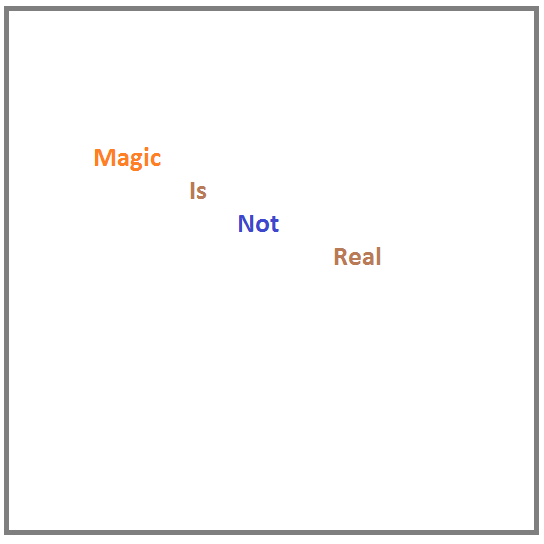
\includegraphics[width=0.5\textwidth]{figs/magic}
\caption{A browser screenshot of Coaster Racer Game.}
\end{figure}

\subsubsection{States}

For the purposes of winning the game, the state of the game at time t is simply the pixel array of the game screen at that particular time. I experimented with using only a cropped version of the game screen that contained the view of the driver. In order to avoid unnecessary computation and memory usage, we downsample this image. By reducing the size of each state, this allows us to fit more training examples in our replay history without running out of memory, which is a crucial component of the experience replay technique we used. In addition, with lower-dimensional input, our network requires fewer matrix multiplications and fewer parameters in the fully connected layers, greatly improving speed.

\begin{itemize}
		
	\item State Space: {Preprocessed screenshots of the browser loading the game}

\end{itemize}

\subsubsection{Actions}

Coaster Racer Flash Game is a typical car racing game which is simply controlled by moving forward, left turn and right turn. With this simple setting, we only only an action space of three actions, namely, moving forward, left turn and right turn.

\begin{itemize}
	
	\item Action Space: {Move Forward action, Turn Left action, Turn Right action}

\end{itemize}

\subsubsection{Rewards}

Rewards are primarily based off of the game score. From the perspective of human player, we judge a good player or not by how the driving behavior is close to real and safe case. While for a Game Bot, it only cares about the score. For this specific game, Coaster Racer Game, it unreasonably encourages a dangerous driving behavior. For example, when the car hits a traffic cone it gets 1000 reward, even if the price of hitting a cone is falling down the road. There is no punishment for falling down the road.

An ideal reward function would encourage the car to stay in the middle of the road and to try not to hitting other cars and guard bars. Here I simply cancel the one time 1000 score reward. But there is still room to fine tune the function in the future.

%%%%%%%%%%%%%%%%%%%%%%%%%%%%%%%%%%%%%%%%%%%
\subsection{Algorithms and Techniques}

\subsubsection{Overal Representation}

\begin{figure}[h]
\centering
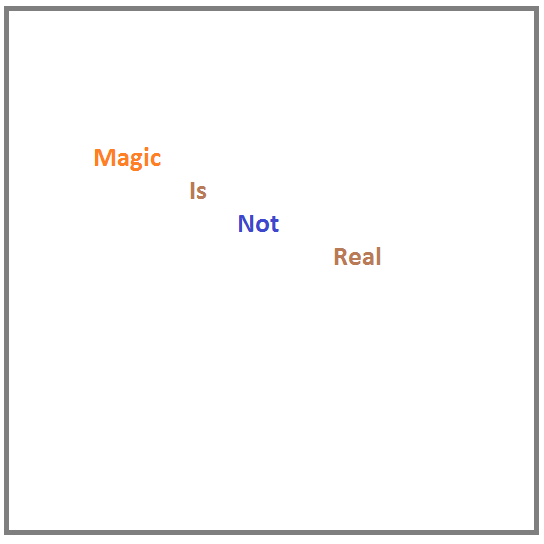
\includegraphics[width=0.5\textwidth]{figs/magic}
\caption{A flowchart of training the Coaster Racer Game Bot.}
\end{figure}

An overall representation of how the different components relate during a play evaluation, centered around the deep Q-network for playing, the main decision component is shown in Figure 3. Each game screen is resized to a desaturated pixels image, and if you might be wondering why each state is a sequence of four game screens instead of one, that is because the agent's history is used for better motion perception. Achieving this requires a sequence of preprocessed images to be stacked in channels (like you would stack RGB channels on a colored image) and fed to the network.

%%%%%%%%%%%%%%%%%%%%%%%%%%%%%%%%%%%%%%%%%%%%%
\subsubsection{Deep Neural Network}
%%%%%%%%%%%%%%%%%%%%%%%%%%%%%%%%%%%%%%%%%%%%%

Convolutional Neural Networks, or CNNs, are a special type of neural network that has a known grid-like topology. Like most other neural networks they are trained with a variant of the back-propagation algorithm. CNN's strength is pattern recognition directly from pixels of images with minimal processing. We use a convolutional network as a function mapping the preprocessed images to Q values, since the actions are highly based on what would be seen as pixel matrix.

\begin{itemize}

	\item \textbf{DeepMind's Deep Q Network}
	
	\begin{figure}[h]
	\centering
	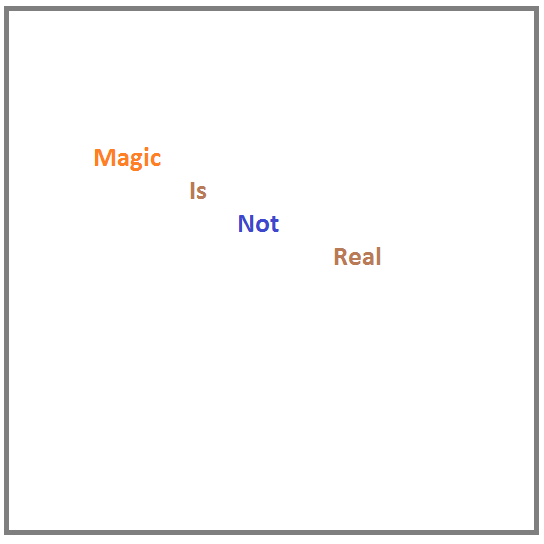
\includegraphics[width=0.5\textwidth]{figs/magic}
	\caption{Deep Neural Network model from DeepMind paper.}
	\end{figure}
	
	The network's architecture that I firstly used is essentially the same used by DeepMind, except for the first convolutional neural network's input (80x80x4 instead of 84x84x4, to account for the different input sizes) and the linear layer's output (3 instead of 18, to account for the different number of actions available).
	
	\item \textbf{LeNet-5.}
	
	\begin{figure}[h]
	\centering
	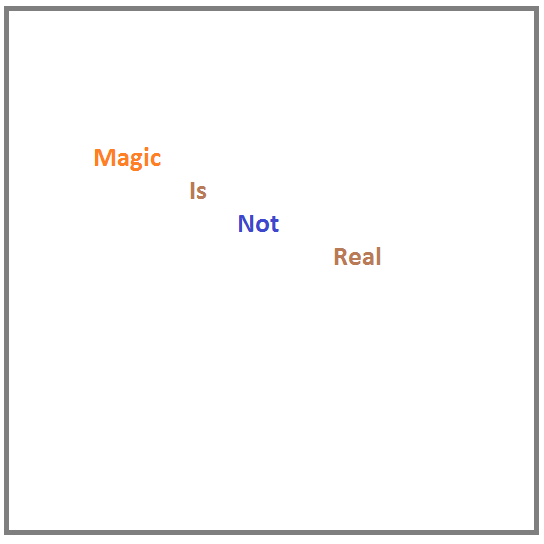
\includegraphics[width=0.5\textwidth]{figs/magic}
	\caption{LeNet-5.}
	\end{figure}
	
	For an image classification problem, there are several mature models other than the one above such as LeNet, VGG, Inception and Xception. I then tried a LeNet-5 model here and expected it to perform better than the DeepMind one for predicting actions. LeNet is deeper than the DeepMind one to grasp more features and has some dropout layers to avoid overfitting. In practice, it shows an advantage especially on predicting turning actions.
	
\end{itemize}

%%%%%%%%%%%%%%%%%%%%%%%%%%
\subsubsection{Q-learning}
%%%%%%%%%%%%%%%%%%%%%%%%%%

One of the most basic and popular methods to estimate action-value functions is the \emph{Q-learning} algorithm. It is model-free online off-policy algorithm, whose main strength is that it is able to compare the expected utility of the available actions without requiring a model of the environment. Q-learning works by learning an action-value function that gives the expected utility of taking a given action in a given state and following a fixed policy thereafter.

A value function estimates what is good for an agent over the long run. It estimates the expected outcome from any given state, by summarizing the total amount of reward that an agent can expect to accumulate into a single number. Value functions are defined for particular policies.

The \emph{state value function} (or V-function), is the expected return when starting in state $s$ and following policy $\pi$ thereafter~\citep{Sutton1998RL},
%
\begin{equation}
V^\pi(s) = \mathbb{E}_\pi \left[R_t | s_t = s \right]
\end{equation}

The \emph{action value function} (or Q-function), is the expected return after selecting action $a$ in state $s$ and then following policy $\pi$,
%
\begin{equation}
Q^\pi(s,a) = \mathbb{E}_\pi \left[ R_t | s_t = s, a_t = a \right]
\end{equation}

The \emph{optimal value function} is the unique value function that maximises the value of every state, or state-action pair,
%
\begin{eqnarray}
Q^*(s,a) & = & \max\limits_\pi Q^\pi(s,a), \forall s \in \mathcal{S}, a \in \mathcal{A}
\end{eqnarray}

An \emph{optimal policy} $\pi^*(s,a)$ is a policy that maximises the action value function from every state in the MDP,
%
\begin{equation}
    \pi^*(s,a) = \argmax_\pi Q^\pi(s, a)
\end{equation}

The update rule uses action-values and a built-in max-operator over the action-values of the next state in order to update $Q(s_t, a_t)$ as follows,

\begin{equation}
Q(s_t,a_t) \gets Q(s_t,a_t) + \alpha \left[r_{t+1} + \gamma \max_a Q(s_{t+1},a) - Q(s_t,a_t)\right]
\end{equation}

The agent makes a step in the environment from state $s_t$ to $s_{t+1}$ using action $a_t$ while receiving reward $r_t$. The update takes place on the action-value $a_t$ in the state $s_t$ from which this action was executed. This version of Q-learning works well for tasks with a small a state-space, since it uses arrays or tables with one entry for each state-action pair.

In this project the policy is using the \textbf{$\epsilon$-greedy} policy:

\begin{itemize}

    \item \textbf{$\epsilon$-greedy.} Selects the best action for a proportion
        $1 - \epsilon$ of the trials, and another action is randomly selected (with
        uniform probability) for a proportion,
        
        \begin{equation}
            \pi_{\epsilon}(s) = \left\{
             \begin{array}{lr}
                 \pi_{\textrm{rand}}(s,a) & \text{if } rand() < \epsilon\\
                 \pi_{\textrm{greedy}}(s,a) & \text{otherwise}
             \end{array}
           \right.
        \end{equation}

        where $\epsilon \in [0, 1]$ and $rand()$ returns a random number from a uniform distribution $\in [0, 1]$.

\end{itemize}

%%%%%%%%%%%%%%%%%%%%%%%%%%%%%%%%%%%%%%%%%%%
\subsection{Benchmark}

This benchmark consists in playing against an agent that takes uniformly random moves. This is the most basic benchmark, but first we have to be sure that our learned evaluation function can play better than a random agent before moving into a harder benchmark. Also, this will help us to detect bugs in the code and algorithms: if a learned value function does not play significantly better than a random agent, is not learning. The idea is to test against this benchmark using Alpha-beta pruning at 1, 2 and 4-ply search.

%%%%%%%%%%%%%%%%%%%%%%%%%%%%%%%%%%%%%%%%%%%%%%%%%%%%%%%%%%%%%%%%%%%%%%%%%%%%%%%%%%%%%%%%%%%%%%%%%%%%





%\bibliographystyle{plainnat}				%Uncomment this if you want a bibliography on each chapter
%\markright{\textit{Bibliography}}
%\renewcommand{\chaptername}{}
%\bibliography{my_references}

%\vfill


\chapter{Methodology}

\section{Section header}

\section{Algorithm}

Q-learning, a model-free online off-policy algorithm, whose main strength is that it is able to compare the expected utility of the available actions without requiring a model of the environment:

\begin{equation}
        Q(s_t, a_t) \gets Q(s_t, a_t) + \alpha [r_{t+1} + \gamma \max_a Q(s_{t+1}, a) - Q(s_t, a_t)]
\end{equation}

%%%%%%%%%%%%%%%%%%%%%%%%%%%%%%%%%%%%%%%%%%%
\subsection{Data Preprocessing}

\begin{itemize}

    \item Crop.
    
    	\begin{figure}[h]
   	 \centering
   	 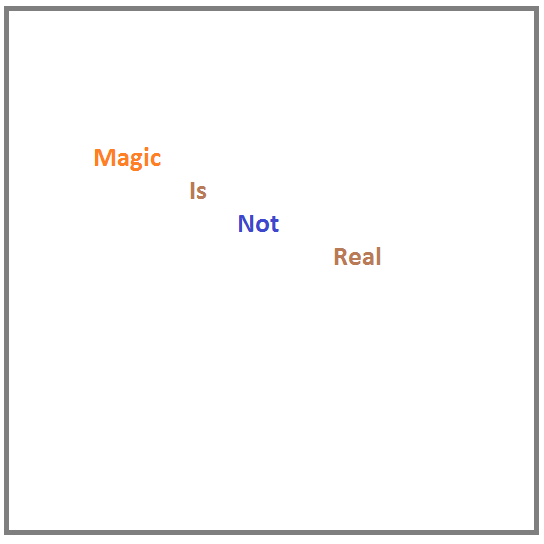
\includegraphics[width=0.5\textwidth]{figs/magic}
    	\caption{Cropped input image.}
    	\end{figure}
    
    The raw input image is captured by Universe in the function "step()" which is simply a screenshot of the browser as shown in Figure 2. Obviously the useful vision information are only from the game screen. If we go further, the top half of the game screen displaying the sky does not change very much and the bottom half of the is heavily effected by the turning actions. Thus a region of interest is carefully chosen by whether considering whether it relates to decide an expected steering behavior.  Then the image is simply cropped by a new window with the "cropFrame()" function. An example cropped image is as shown in Figure 6.   
    
    \item Downscale the resolution.

    	\begin{figure}[h]
    	\centering
   	 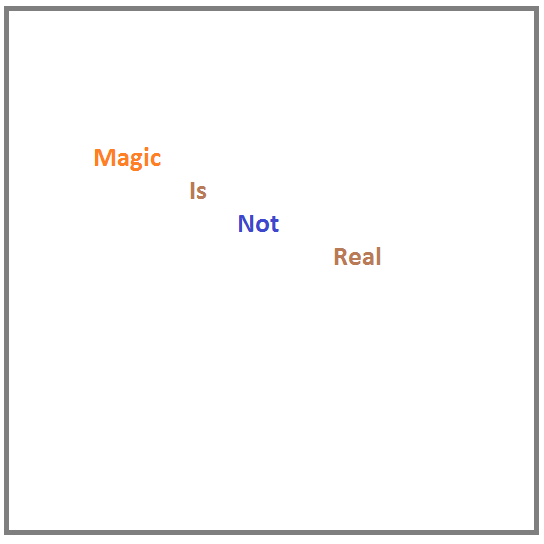
\includegraphics[width=0.25\textwidth]{figs/magic}
   	 \caption{Downsized input image.}
    	\end{figure}
    
    A high resolution is usually redundant for a computer vision task. By resizing with a smaller size, the space information are almost remained and the computing time are greatly saved. The cropped image is then downsized to a smaller size, [80, 80] as in Figure 7. Downscaling the resolution doesn't hurt the information for turning left or right but highly accelerating the computing since much smaller data are being processed.
    
    \item Grayscale.

	\begin{figure}[h]
	\centering
	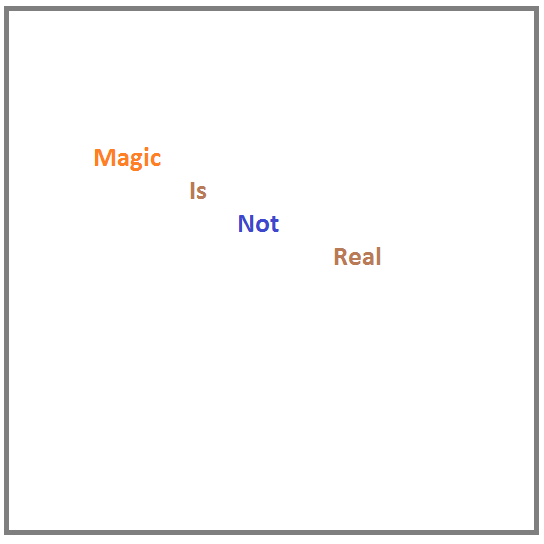
\includegraphics[width=0.25\textwidth]{figs/magic}
	\caption{Grayscaled input image.}
	\end{figure}
    
   Grayscale processing is another useful technique in computer vision tasks since it is a great help for accelerating the computing and is at least three times faster than that of color image processing. This is because grayscale image has only one color channel as opposed to three in a color image.  The color information are usually dumped when unnecessary for the computer vision tasks. As here, the downsized image is gray scaled as in Figure 8, because the color information does not help much for the steering control. 

\end{itemize}

%%%%%%%%%%%%%%%%%%%%%%%%%%%%%%%%%%%%%%%%%%%
\subsection{Implementation}

\subsubsection{Environment Setting}

OpenAI Universe is designed with using Docker so it can reset the Game continuously. Docker is a tool that lets you run virtual machines on the local computer. I created an image wrapping up everything necessary, like TensorFlow, OpenCV, Gym and Universe.

To start up a very first Game Environment, only gym and universe modules are needed. Since we are to generate some random behaviors, "random" is also imported.

...

\subsubsection{Build the Deep Neural Network}

The Deep Neural Network is based on the DeepMind paper except for the changes of input and output sizes.

...

\subsubsection{Preprocessing Functions}

As described in the previous chapters, the crop, downsample and grayscale operations are done with the following functions:

...

\subsubsection{Finetuning Hyperparameters}

I played with some hyperparameters:

\begin{itemize}
\item The number of time steps
\item The capacity of the replay memory,
\item The layers of the network and the region of interest.
\end{itemize}
Currently this process is nothing more than trial and error. I could be better designed by grid search or random search. Well, it could be even easier to design the pipeline of implement a Deep Reinforcement Learning problem but tougher in hyperparameter tuning. Without a deeper understanding of the features of model, it has a high probability to fall into a less efficient experiment process. 

%%%%%%%%%%%%%%%%%%%%%%%%%%%%%%%%%%%%%%%%%%%
\subsection{Refinement}

\subsubsection{Relay Memory}
Along the first several trials, I experimented with different memory capacities. The memory is a pool where the Game Bot would pick actions by Q values from. A small pool means it would be quick to converge during the training stage while it also limits the capacity it can learn. So there is a tradeoff here.

\subsubsection{The Complexity of the Nerwork}
The original works well for some simple game such as Atari and CartPole. The Coster Racer Game here is more complex to play because it scores by driving along the way with a high speed. The delay between an action and a reward is bigger. Through a long time training, it has a bad classification on Left Turn and Right Turn cases.

I replace the DeepMind model with LeNet-5 which then shows a better ability in classifying and quicker convergence.



%\bibliographystyle{plainnat}
%\markright{\textit{Bibliography}}
%\renewcommand{\chaptername}{}
%\bibliography{KL-Thesis}

%\end{flushleft}
%\vfill

\chapter{Results}
 
\section{Specimen Selection \& Characterization}

\subsection{Model Evaluation and Validation}

\begin{figure}[h]
\centering
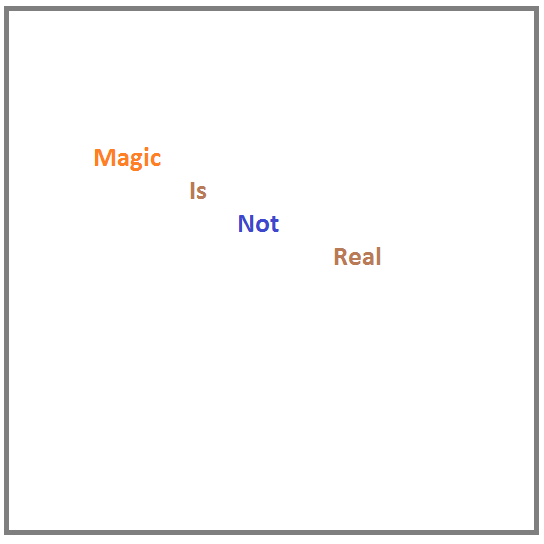
\includegraphics[width=0.5\textwidth]{figs/magic}
\caption{High score by the Game Bot.}
\end{figure}

Figure 9 is a screenshot when the car reach the finishing line and it got a score of 10269. The network was trained over 10,000 time steps and the behavior has been learned gradually. Compared to random bot, it has shown obvious better performance. For better or human level behavior, more training time steps are needed.

%%%%%%%%%%%%%%%%%%%%%%%%%%%%%%%%%%%%%%%%%%%%%%%%%%%%%%%%%%%%%%%%%%%%%%%%%%%%%%%%%%%%%%%%%%%%%%%%%%%%
\subsection{Justification}

\begin{figure}[h]
\centering
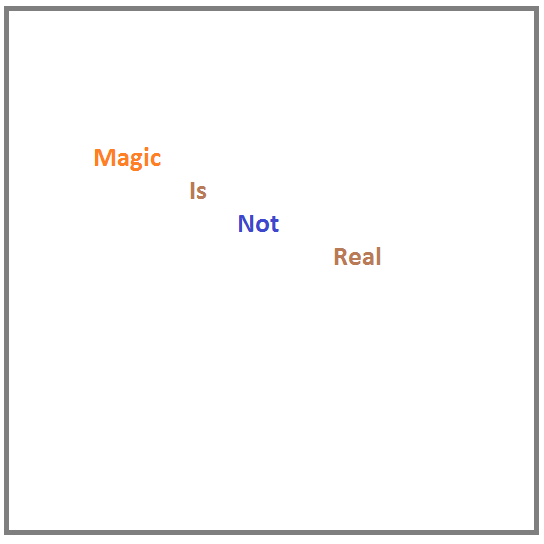
\includegraphics[width=0.5\textwidth]{figs/magic}
\caption{A comparison between DQN trained Game Bot and a random Game Bot.}
\end{figure}

The reward histories shown in Figure 10 indicates how it performs better than a random Game Bot when the DQN one is trained 100000 time steps. It proves a much better ability to earn scores or rewards though there is still a big room to improve. The Game Bot can earn as high as 10269 scores though it still usually ranks the last.


%\bibliographystyle{plainnat}
%\markright{\textit{Bibliography}}
%\renewcommand{\chaptername}{}
%\bibliography{my_references}


\vfill

%Discussion
\chapter{Discussion}





%\vfill

%Conclusions
\chapter{Conclusions}

\subsection{Free-Form Visualization}

A Youtube video has also been uploaded with the link https://youtu.be/VdVA3od4tVs here and it shows how it performs after 17000 time steps' training. It shows a capacity to stay in the road though it has some difficulty choosing right actions when blocked by the guard bars. The guard covered part of its view and the always acceleration actions made it even hard to get out of the stuck.

%%%%%%%%%%%%%%%%%%%%%%%%%%%%%%%%%%%%%%%%%%%
\subsection{Reflection}

\subsubsection{Diffculties}

The most difficult aspect of this project was that is extremely hard to stabilize reinforcement learning with non-linear function approximators. There are plenty of tricks that can be used and hyper-parameters that need to be tuned to get it to work, such as exploration policy, discount factor, learning rate, number of episodes, batch size, experience pool size and initial value.

All these techniques and parameters were selected by trial and error, and no systematic grid search was done due to the high computational cost. More than once it seemed that the implementation of the algorithms and techniques was incorrect, and it turned out that the wrong parameters were being used. A ``simple'' change such as decreasing $\epsilon$, or changing the neural network optimizer made big changes in the performance of the value function.

Also a huge difficulty of a reinforcement learning problem could be the time lag between the action and the reward. When training with grouped actions off of the heuristic reward function, the reward for a given action was immediate, and this network showed the best performance. The next best performance came from a network based off of grouped actions, where actions were only a few steps removed from the next reward. Our worst performance came from the networks trained to estimate actions, where actions were several dozen steps removed from the next rewards.

\subsubsection{General Pipeline}

In a Deep Q Network setting, there are several elements which we have to be careful to define.

\begin{itemize}
	
    \item \textbf{Environment:} An environment defines what the agent interacts with. It receives states and actions and generate new states and plays a role as an online data generator. 
    \item \textbf{State Space:} A state is the input of the Deep Q Network. In this project, the stats is an image or a pixel array. It will be trained by a Deep Neural Network and predict the next actions.
    \item \textbf{Action Space:} An action space could be discrete and continuous. It defines the all classes that would be generated from the Deep Q Network. A bigger action space indicates a bigger room for an agent to learn and improve but also means a much complexity to train.
    \item \textbf{Reward Functions:} The reward function determines in which way we would like the agent to grow. For example, we would define a bigger reward for the car to stay in the middle of the road than in the side of the road. It can be a discrete or a continuous function.
    \item \textbf{Deep Neural Network:} The Deep Neural Network is responsible to map the states to the Q values, which are corresponding to different actions by Q functions. 
    \item \textbf{Fine tune the Hyperparameters:} By fine tuning the hyperparameters, we try to maximize the ability of the defined Deep Q Network. It can be subtle to modify the hyperparameter values which might change the output in different ways, like effecting the time of the convergence, the prediction accuracy, overfitting or underfitting and robustness.
    
\end{itemize}






%\vfill

\chapter{Future Work}

Given this thesis mainly covers the basic Deep Q-Learning algorithm, it leaves plenty of room for further exploration into the fancier algorithm. The admin/base layer will need to prevent user interference and act as a ?final check? to algorithm and control commands that the user level wishes to execute. The user layer will need to allow users to integrate their computers, sensors, and other hardware into the user level and allow them to control their tests. A study on sensor fusion and techniques can be carried out to determine the optimal method for continuous integration and fusion of added LIDARs, radars, and other sensors. Development of a Hardware-In-the-Loop (HIL) simulation environment can greatly help to expedite testing and verification of researchers? tests before they are carried out.

For future work on hardware, an analysis and testing of several different brands and models of LIDAR, radar, ultrasonic, and cameras can be carried out. This will further assist in determining what actual products will be adequate for the scope of the platform to be developed, particularly what is best to outfit the base sensor suite with. Research into developing a standard platform conversion kit that could be adaptable to a variety of autonomous base vehicles would be great for bringing research platform capability to those who want it.

For an AVRP, technology will always be improving and the needs of the researcher will always be varying and changing. This in turn will require constant research and learning in order to keep the systems of an AVRP up to date and functional for its users.

\section{Improvement}

There are at least two aspects we can improve in the next stage,

\begin{enumerate}

    \item \textbf{Tuned Reward Functions:} In this thesis, the learning process is highly relying on the difenition of the reward function.
    
    \item \textbf{Better benchmarks:} In most of this thesis we used simple benchmarks, such as playing against random players. While testing against random is probably the first thing to test against (if you can't beat a random player your learning algorithm is not working), it would be better to find a few heuristics and better players that can be used for testing.

    \item \textbf{Incorporate other RL techniques:} The field of RL has been advancing fast in recent years. There are a few new and old techniques that I would like to try, such as asynchronous RL, double Q-learning, prioritized experience replay and Asynchronous Actor-Critic Agents (A3C).

\end{enumerate}

%\include{10-Summary}
\appendix
\chapter{Pprofile}
Here is a section for HHP profile stuff, whatever that is...

\begin{itemize}
\item Pprofile 1 stuff here
\item Pprofile 2 stuff here
\item Pprofile 3 stuff here
\item Etc...
\end{itemize}

 % HHP profile
\chapter{Specimens}
Here is a section to describe specimens used in this research.

\begin{itemize}
\item Specimen 1 stuff here
\item Specimen 2 stuff here
\item Specimen 3 stuff here
\item Etc...
\end{itemize}

 % master list
\chapter{Preparation of this document}
This document was prepared using pdf\LaTeX\ and other open source tools. The (free) programs implemented are as follows:

\begin{itemize}
\item \LaTeX\ implementation:\\
  \textbf{MiK\TeX}\\
  \href{http://www.miktex.org/}{http://www.miktex.org/}\\
  \textbf{\TeX}\textbf{Live}\\
  \href{https://www.tug.org/texlive/}{https://www.tug.org/texlive/}\\
  \textbf{Mac}\textbf{\TeX}\\
  \href{https://tug.org/mactex/}{https://tug.org/mactex/}\\
\item \TeX-oriented editing environments:\\
  \textbf{Vim Text Editor}\\
  \href{https://http://www.vim.org/}{https:http://www.vim.org/}\\
\item Bibliographical:\\
  \textbf{Bib}\textbf{\TeX}\\
  \href{http://www.bibtex.org/}{http://www.bibtex.org/}\\
  \textbf{Zotero}\\
  \href{https://www.zotero.org/}{https://www.zotero.org/}\\
\end{itemize}
 % programs used to generate this document
\chapter{Figures}
Here is a section for figures in the document.

\begin{itemize}
\item Figure 1 stuff here
\item Figure 2 stuff here
\item Figure 3 stuff here
\item Etc...
\end{itemize}

 % list of microscope figures used in text

% To have a bibliography for the whole document, plus individual bibs,
% put \bibliography commands in the included chapters plus in the root
% file; use \usepackage[rootbib]{chapterbib}; run LaTeX; run BibTeX on
% the root file; change to \usepackage{chapterbib}; run LaTeX; run
% BibTeX on each included file; run LaTeX; run LaTeX. An `overall'
% bibliography only makes sense for various `named' bibliography
% styles; a style with numbering will give separate and unrelated
% numbers in each bibliography.
\renewcommand{\bibname}{Complete References}
\bibliographystyle{unsrt} %if you have problems with the style, consult the CWRU-thesis.cls file
\markright{\textit{Bibliography}}
%\renewcommand{\chaptername}{}
\bibliography{refs/my_references}
%if latex throws errors with the .bbl file, fix the problem in the .bib, and delete the .bbl before trying to recompile
%also, if the tex runs but says bib?, you can hit enter and get everything but the bibliography

%\end{document}
%\end


%%% Local Variables: 
%%% mode: tex-pdf
%%% TeX-master: t
%%% End: 


%\documentclass{article}
%\usepackage{units} %For use of \nicefrac{}{} to create units
%\usepackage{fixltx2e} %For use of \textsubscript{}

%%To widen the text columns from the default 'article' settings:
%\setlength{\hoffset}{25pt}
%\setlength{\marginparwidth}{0pt}
%\setlength{\oddsidemargin}{0pt}
%\setlength{\textwidth}{400pt}

%\begin{document}

%\title{Acrylic Durability for Long-Lived Low-Cost PV Systems}
%\author{Myles Murray}
%\maketitle
%\newpage
%\tableofcontents
%\newpage 
%


%\enddocument
\end{document}

				


